\section{Reduction to a weak order}
\label{tree:POP:reduction}


The reduction is achieved through a graph coloring greedy algorithm and a flow algorithm.

To reduce from a partial order to a weak order we need to regroup incomparable elements (stable subsets in $\text{G}(P)$) of the Hasse diagrams into antichains.

\begin{figure}
	\centering
	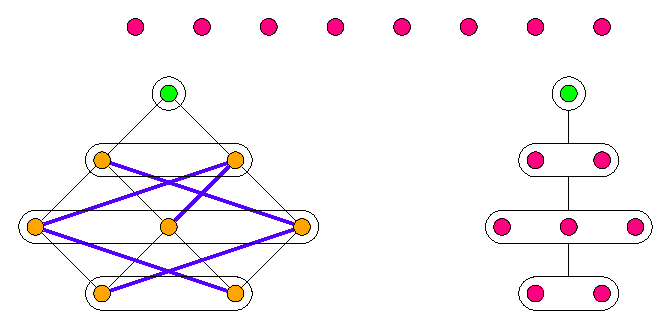
\includegraphics[width=0.8\textwidth]{fig/partial-order-production-reduction:diag}
	\caption{\label{fig:partial-order-production-reduction:diag} Reduction from a partial order production problem to a weak order production problem.}
\end{figure}

\cite{jcardin1} explains that in order to achieve the reduction we cannot stop just after the first run of the greedy coloring algorithm. In deed, there could be some antichains that cross each others.

In order to fix this \cite{jcardin1} runs a flow algorithm based on \ref{eq:entropy:graph}.

The coloring algorithm is then run a second time to produce the final weak order.